\documentclass{article}
\usepackage[utf8]{inputenc}

\title{Random Forests}
\author{Sylesh Suresh and Mihir Patel}
\date{September 2017}

\usepackage{graphicx}

\begin{document}

\maketitle

\section{Overfitting}
\begin{center}
    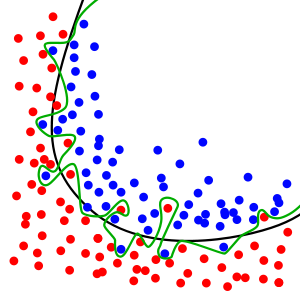
\includegraphics[scale=0.4]{overfitting.png}
\end{center}
Before we cover random forests, we will firstly describe overfitting. The goal of our models is to learn the generalize pattern in data. However, by nature, our data has some random noise. If we look at the image above, we can clearly see the black line represents the semantic separation of the data but some points are misclassified. By contrast, the green line perfectly separates the data, but clearly is abusing the data points that are shifted due to noise. Our goal is to prevent overfitting, which is the green line and maintain our separation on the black line. 

\subsection{Identifying overfitting}
\begin{center}
    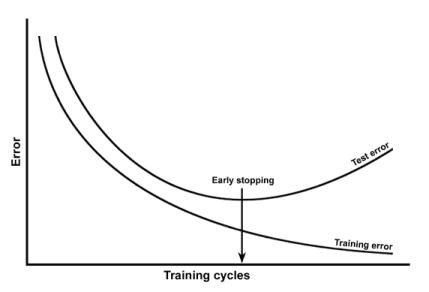
\includegraphics[scale=1.1]{overfittinglines.png}
\end{center}
We can identify overfitting by seeing increases in loss / error for validation data. If the training loss continues to go down, but testing for the generalizable pattern (the validation data) goes up, we have a problem!

\section{Regularization}
The most common technique used to prevent overfitting involves regularization. Essentially, some random noise is added to our model in order to prevent it from being overly tuned to the data. When we adjust parameters in the model, some adjustment is also made that is mostly random. In decision trees, this involves selecting random thresholds and selecting the best one of this set instead of calculating the ideal threshold. This accelerates training and minimizes cases where a threshold is picked to fit a specific case. However, this is often too much noise so isn't commonly used.

\subsection{Restricting Depth}
\begin{center}
    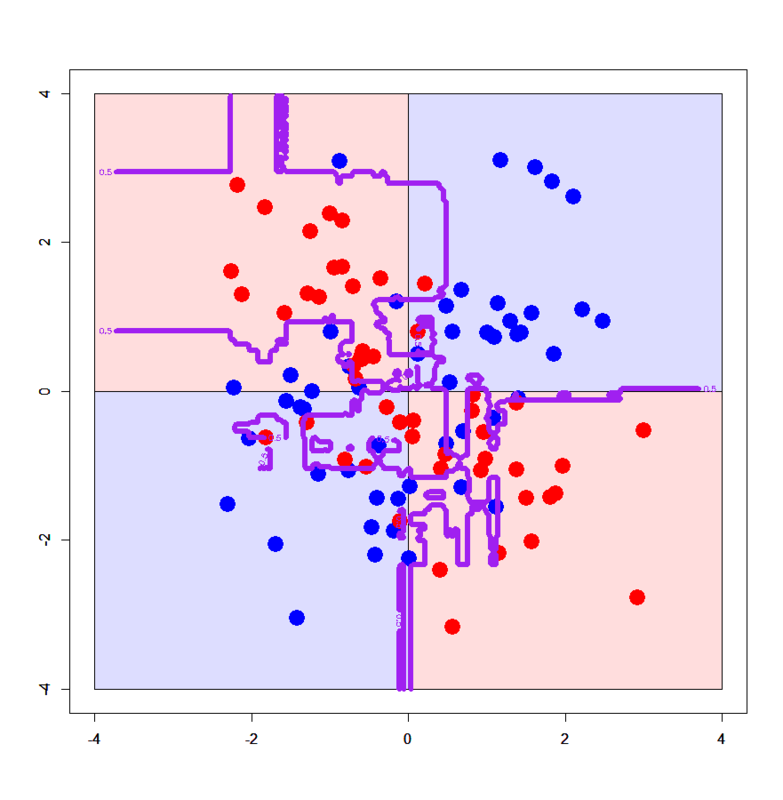
\includegraphics[scale=0.3]{decisiontreeoverfit.png}
\end{center}
In decision trees, the most common approach involves limiting the depth of the trees. For example, it is likely that the last node in the tree focuses on an ad hoc case where one data point causes issues. As seen in the image, we see that the decision tree creates odd lines for specific points. By restricting the depth, we prevent these ad hoc nodes.

\section{Introduction}
Random forests are an ensemble of decision trees, combining many weak learners to build a robust, strong learner that generalizes better to unseen data than the individual weak learners. 

\section{Building a Random Forest}
\begin{enumerate}
    \item Randomly choose $n$ samples from the training set with replacement (i.e. draw a bootstrap sample of size $n$).
    \item Build a decision tree using the bootstrap sample. At each node:
    \begin{enumerate}
        \item Randomly select $d$ features without replacement.
        \item Split the node using the feature among the $d$ features previously selected that provides the best split by maximizing the information gain.
    \end{enumerate}
    \item Repeat steps 1 to 2 $k$ times
    \item Aggregate the prediction by each tree by majority vote to assign the final class label.
\end{enumerate}
Note that when building the decision trees, instead of evaluating all features to find the best split, we select the best feature among only a randomly chosen subset of those features. This creates more diversity among the trees, helping to prevent overfitting. Because of these overfitting-preventative measures, it is not necessary to prune the trees. Individually, each decision tree would perform poorly, but the aggregate of many of these trees leads to a model with a much higher performance.

\subsection{Hyperparameters}
The most important hyperparameter to be optimized here is $k$, the number of decision trees the random forest uses. Although more trees increase the performance of the classifier as a whole, they also increase the computational expense. The hyperparameters $n$ and $d$ can also be optimized. The bootstrap sample size $n$ correlates with the degree of overfitting; larger values of n decrease the randomness, increasing the likelihood of overfitting while smaller values of n increase the randomness at the cost of the model's performance. A good balance is to set $n$ to the size of the training set. Similarly, the size of the feature subset $d$ must be less than the number of features in order to promote diversity among the trees, but must be large enough to not reduce the model's performance. A common convention is to set $d$ to the square root of the number of features. 

\subsection{Extra-Trees}
Instead of searching for the best threshold at each split when building each decision tree, another option is to randomly choose thresholds for each feature of the chosen feature subset and choose the best one from these. This further prevents overfitting at the cost of performance. A random forest built this way is called an Extremely Randomized Trees, or Extra-Trees.

\section{Feature Importance}
Random Forests can be helpful in ranking and evaluating feature importance. In an individual decision tree, intuitively, the most important features are split near the root of the tree while less important features are either split near the leaf nodes or are not split at all. In other words, the depth of a feature in a decision tree gives a measure of the importance of that feature. In a random forest, one can take advantage of this property by taking the average depth of a feature across all the individual trees to measure its importance. 
Here is an example of a random forest ranking the importance of pixels in a face recognition problem where the brighter pixels are more important:

\begin{center}
    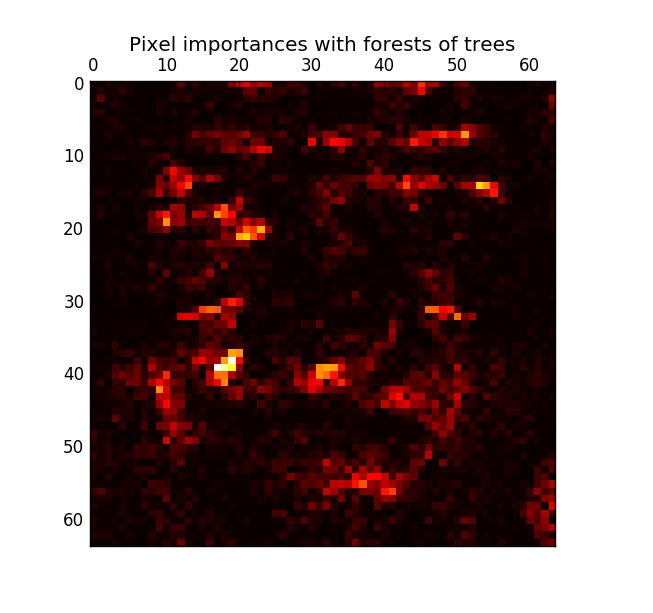
\includegraphics[scale=.4]{featureimportance.jpg}
\end{center}

\end{document}
